\label{chap:theory}

This chapter will introduce some basic theory needed to develop our approach to user modeling.
We will first describe our stated enemy, the information overload problem, before delving into
how user modeling and, more specifically, recommender systems, is currently used to solve this problem.

This chapter will also introduce the notion of personalized search, a field where
our user modeling method will be especially applicable.
The next chapter will use these theories to build an 
a method for \emph{adaptive prediction aggregation}
called \emph{stacked user modeling}.

\section{Information Overload}

Information overload conveys the act of receiving \emph{too much information}. 
The problem is apparent in situations where decisional accuracy turns from improving with more information, to being hindered by too much irrelevant data \cite[p13]{Bjorkoy2010d}. 
Needness to say, this is a widespread phenomenon, with as many definitions as there are fields experiencing the problem. Examples include \emph{sensory overload}, \emph{cognitive overload} and \emph{information anxiety} \citep{Eppler2004}.

Two common tasks quickly become difficult in this situation:
Consuming content that is known by the user to be relevant can be drowned out by irrelevant noise.
Orthogonally, discovering new, interesting yet unknown content also becomes difficult because of the sheer amount of available content.
Finding contemporary examples is not difficult:

\begin{itemize*}
  \item Missing important news articles that get drowned out by irrelevant content.
  \item Forgetting to reply to an email as new messages keep arriving.
  \item Discovering sub-par movies because those most relevant are never discovered.
\end{itemize*}

The overload is often likened to a \emph{paradox of choice}, as there may be no problem acquiring the relevant information, but rather identifying this information once acquired. As put by \cite{Edmunds2000}: "The paradox --- a surfeit of information and a paucity of useful information."
While normal cases of such overload typically result in feelings of being overwhelmed and out of control, \cite{Bawden2008} points to studies linking extreme cases to various psychological conditions related to stressful situations, lost attention span, increased distractibility and general impatience.

\cite{Kirsh2000} argues that "the psychological effort of making hard decisions about \emph{pushed} information is the first cause of cognitive overload." 
According to \citeauthor{Kirsh2000}, there will never be a fully satisfiable solution to the problem of overabundant information, 
but that optimal environments can be designed to increase productivity and reduce the level of stress through careful consideration of the user's needs. 
In other words, to solve the problems of information overload and content discovery, applications must be able to individually adapt to each user. 

An insightful perspective on information overload comes from the study of attention economy. 
In this context human attention is seen a scarce commodity, offset by how much irrelevant noise is present at any given time. 
Attention can then be defined as "... focused mental engagement on a particular item of information. 
Items come into our awareness, we attend to a particular item, and then we decide whether to act" 
\citep{Davenport2001}. 
To evade information overload is then to maximize available attention, allowing more focus on the most important items of an interface.

\begin{wrapfigure}{rt}{0.4\textwidth}
  \vspace{-20pt}
  \begin{center}
    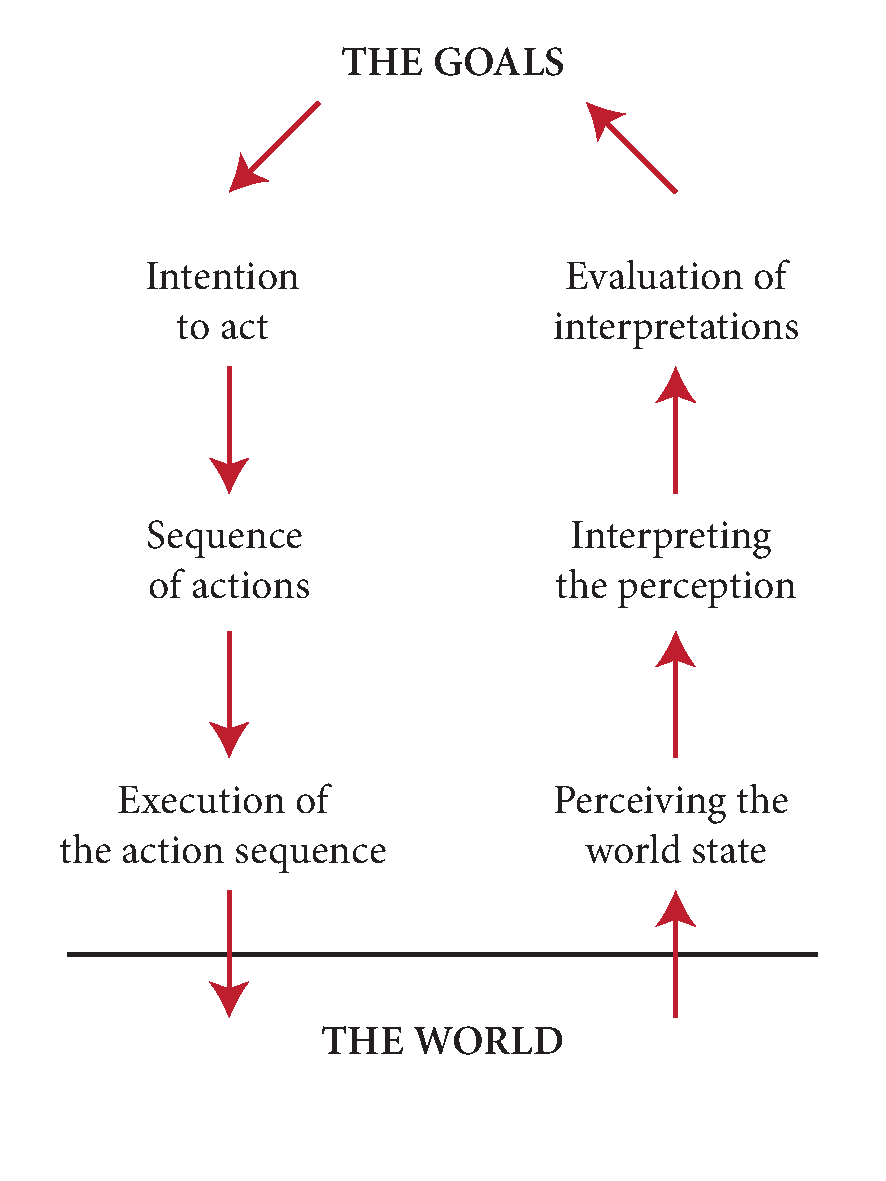
\includegraphics[width=0.4\textwidth]{../graphics/seven-stages.pdf}
    \vspace{-20pt}
    \caption[The Seven Stages of Action]{}  
  \end{center}
  \label{fig:seven-stages}
  \vspace{-30pt}
\end{wrapfigure}

Conceptual models used in interaction design can help us see when and where information overload interferes with the user experience. 
\cite{Norman1988} advocates a model called the seven stages of action, describing how each user goes through several states while using a system
(see Figure \ref{fig:seven-stages}). 
First, the user forms a goal and an intention to act. The user then performs a sequence of actions on the world (the interface)
 meant to align the perceived world and the goals. After performing a set of actions, the new world state is evaluated and perceived. 
At last, the user evaluates the perception and interpretation of the world in accordance with the original goal.

As apparent from this model, information overload can interfere both before and after any action is taken. 
For example, if the application presents too much content, or presents content in a confusing manner, 
it can be difficult for the user to identify which actions that would help achieve the current goal. 
Likewise, after actions are taken, the new world state can suffer the same shortcomings of overwhelming scope or lack of presentations, 
leading to information overload. 
This precludes the user from properly evaluating the resulting application state. 

In short, an application interface can fail both before and after a user tries to interact with it.
Information overload happens throughout the interaction process, which is important to know when considering possible solutions.

\subsection{Online Overload}

The Web is a common source of information overload. 
As we will use the web as an example throughout this paper, 
this section describes why the Web is so conducive to information overload.

Online information overload is especially pervasive when considering \emph{content aggregating websites}, 
i.e. sites that collate information from multiple other sites and sources. 
Online information retrieval (i.e. search engines), fall into this category, as does
online newspapers, feed readers and portal websites.
As mentioned, the wealth and scope of data are natural culprits of online overload, 
as well as the varying qualities of websites publishing the information. 
However, lessons from graph theory can also help us see why information overload occurs on the Web.

Graph theory presents applicable models of the Web that characterize how people navigate between websites, 
and show how content aggregators form important hubs in the network. 
These models also show a theoretical foundation for why information overload occurs.
In the Web graph, nodes correspond to websites and
directed edges between nodes are links from one page to another. The \emph{degree} of a node is defined as its number of edges.

The Internet has the properties of a \emph{small-world network} \citep{Newman2000}, 
a type of random graph, where most nodes are not neighbors, but most nodes are reachable through a small number of edges (See Figure \ref{fig:swn}). 
This is because of important random shortcuts differentiating the graph from a regular lattice. 
The graph is not  random, but neither is it completely regular.
As described by \citet[p37]{Barabasi2003}, the average number of outbound links from a webpage is around 7.
From the first page, we can reach 7 other pages. From the second, 49 documents can be reached. 
After 19 links have been traversed, about $10^{16}$ pages can be reached (which is more than the actual number of existing web pages, since loops will form in the graph).
%\footnote{The concept of small-world networks came from the observation that there is often a surprisingly short minimum distance between nodes in an average graph. This is called the small world phenomenon, and is often mentioned alongside the concept of "six degrees of separation", popularized in a play by John Guare. This concept states that no person is on average more than six social links removed from any other person on earth.}

\begin{figure}[t]
  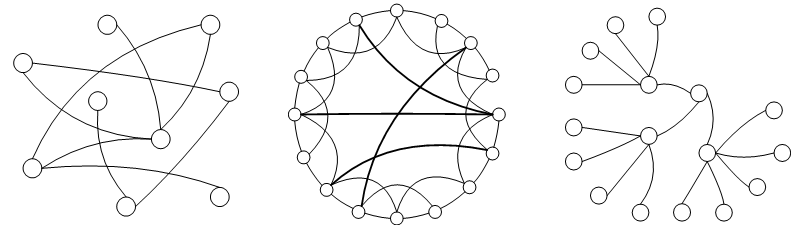
\includegraphics[width=\textwidth]{../graphics/graphs}
  \caption[Complex Networks]{
    Complex Networks,
    from the left: A \emph{random} network, a \emph{small-world} network and a \emph{scale-free} network 
    (which is a type of  small-world network). Figure adapted from \cite{Huang2005}.} 
  \label{fig:swn}
\end{figure}

The high degree of the Web graph would suggest that finding an optimal path to your desired page is quite difficult. 
Yet, while it is true that finding the \emph{optimal path} is hard, finding \emph{a good path} is not that big a challenge. 
When people browse the Web, links are not followed blindly --- we use numerous different heuristics to evaluate each link, often resulting in a quite good path to where we want to go. 
So why is the Web still quite challenging to navigate?

As discovered by \cite{Albert1999}, the Web also exhibits properties of a \emph{Scale-Free Network} (\smallcaps{SFN}). 
They found that in some natural observed networks, there exists a small number of nodes with an extremely high degree. 
This is also true on the Web --- some websites have a huge number of outbound links. 
For comparison, while a random network is similar to a national highway system, with a regular number of links between major cities, scale-free networks are more like an air traffic system, with central hubs connecting many less active airports \citep[p71]{Barabasi2003}.

These highly connected nodes, called \emph{hubs}, are not found in small-world networks or random graphs. As demonstrated by the presence of hubs, the degree distribution of a scale-free network follows a power law, 
$P(k) \sim k^{-\gamma}$, 
where $P(k)$ is the probability of a node having k connections and $\gamma$ is a constant dependent on the type of network, typically in the range $2 < \gamma < 3$. 
Since the Web has directed edges,
we have two power laws:
$P_{in}(k) \sim k^{-\gamma_{in}}$ and 
$P_{out}(k) \sim k^{-\gamma_{out}}$.

\cite{Albert1999} describes a number of studies placing the $\gamma$ values for the Web in the $[2,3]$ range, 
with $\gamma_{out}$ being slightly higher than $\gamma_{in}$. 
Both these probabilities exhibit power tails (or long tails). 
In other words, a few important nodes have a huge number of inbound and outbound links --- the hubs. 
\citet[p86]{Barabasi2003} proposed that hubs emerge in a scale-free networks because of two factors:
(1) Growth: Nodes are added to the network one by one, for example when new websites are added to the Internet.
(2) Preferential attachment: When new nodes are created, they connect to existing nodes. The probability that the new node will connect to an existing node is proportional to the number of links the existing node has. In other words, older, more established and central nodes are preferred neighbors.

This is called the Barab\'{a}si-Albert model \citep{Albert1999}, 
and the probability for a new node connecting to an existing node is given by $\prod k_i$ in Equation \ref{eq:albert:prob}, 
where $k_i$ is the number of links pointing to node $i$. 

\begin{equation}\label{eq:albert:prob}
  \prod_{i} k_i  = \frac{k_i}{\sum_{j}^N k_j}
\end{equation} 

\vspace{1em}
\noindent
Another important topological observation of the Web is how fragmented it is. 
\citet[p166]{Barabasi2003} describes the Internet as a number of continents:

The first continent is the \emph{central core}, where most important hubs reside. On this continent, most sites are easily reachable through each other.
The second is the \emph{in-continent}, and is defined by the group of websites that often link to sites in the central core, but seldom receive reciprocal links from central hubs.
The third is the \emph{out-continent}, which are comprised of sites that are often linked to from the central hub, but seldom link back.
Finally, the Internet has many \emph{islands}, or dark nets, which are not accessible through links from other continents. 
The islands of the Web is why search engines allows web masters to manually add their sites to the search engine index --- not all sites are discoverable by following simple links. Some of the Web is topographically close, but a lot of it is not.

Returning to our main topic, the \emph{hubs} often represent the previously mentioned \emph{content aggregating websites}. 
Search engines, social link aggregators, news portals, et cetera are all hubs of the Internet, emerging from the preferential 
link attachment of newly created nodes. 
Factor in the existence of multiple sub-graphs, or continents, and we can intuitively see that navigating the Web is not as 
easy as it might appear from simple models.

What does seem clear is that these content aggregating hubs are prime candidates for overwhelming their users with information. 
The fundamental observed structure of the Web creates the need for information brokers that link the net together, 
and the need for techniques to display a lot of data. 

So far we have established that information overload is a pervasive problem, especially on the web.
The question now becomes how to best solve this issue. 
This is where user modeling comes in.



\section{User Modeling}
\label{sec:modeling}

The term \emph{user modeling} (\smallcaps{UM}) lacks a strict definition. 
Broadly speaking, when an application is adapted in some way based on what the system knows about its users, we have user modeling. 
From predictive modeling methods in machine learning, 
to how interface design is influenced by personalization --- the field covers a lot of ground. 

It is important to differentiate between adapting the interface of an application and the content of an application. 
Many user modeling methods strive to personalize the interface itself, e.g. menus, buttons and control elements 
(e.g. \cite{Jameson2009, Fischer2001}. 
Adapting the application content, on the other hand, means changing how and what content is displayed
For instance, interface adaption might mean changing the order of items in a menu, while content 
adaption might mean changing the order and emphasis of results in a web search interface
(e.g. \cite{Xu2008, Qiu2006, Rhodes2000}).

In this thesis, we are interested in adapting the \emph{content} of an application.
The source of information overload problem often comes down to a mismatch between presented content and desired content. 
Examples of this kind of user modeling include:

\begin{itemize*}
  \item Suggesting interesting items based on previous activity.
  \item Reorganizing or filtering content based on predicted user relevance.
  \item Translating content based on a user's geographical location.
  \item Changing the presentation of content to match personal preferences or abilities.
  \item Personalizing search results based on previous queries and clicks.
\end{itemize*}

The fields of Artificial Intelligence (AI) and Human-Computer Interaction (HCI) share a common goal solving information overload through user modeling. 
However, as described by \cite[p6]{Lieberman2009}, they have different approaches and their efforts are seldom combined: 
while AI researchers often view contributions from HCI as trivial cosmetics, the HCI camp
tends to view AI as unreliable and unpredictable --- surefire aspects of poor interaction design.

In AI, user modeling refers to precise algorithms and methods that infer knowledge about a user based on past interaction 
(e.g. \cite{Pazzani2007, Smyth2007, Alshamri2008, Resnick1994}).
By examining previous actions, predictions can be made of how the user will react to future information. This new knowledge is then embedded in a model of the user, which can predict future actions and reactions. 
For instance, an individual user model may predict how interesting an unseen article will be to a user, based on previous feedback on similar articles or the feedback of similar users.

HCI aims to meet user demands for interaction. 
User modeling plays a crucial role in this task. 
Unlike the formal user modeling methods of AI, user models in HCI are often cognitive approximations, manually developed by researchers to describe different types of users 
(e.g. \cite{Fischer2001, Jameson2009, Cato2001}).
These models are then utilized by interaction designers to properly design the computer interface based on a models predictions of its user’s preferences.
\cite{Totterdell1990} describes user modeling in interaction design as a collection of deferred parameters: "The designer defers some of the design parameters such that they can be selected or fixed by features of the environment at the time of interaction [...] Conventional systems are special cases of adaptive systems in which the parameters have been pre-set."

This thesis is concerned with the AI approach to user modeling, and in particular, the use of \emph{recommender systems} (RSs).
As our goal is to combine different RSs into one coherent user model, 
we shall now describe what makes a recommender system,
and introduce some of the many algorithms they employ.



\section{Recommender Systems}
\label{sec:recommender}

While the name might seem constraining, recommender systems are incredibly powerful methods in user modeling.
Whenever we wish to predict the relevance of an item to a user, recommender systems are the tools to use.
Such systems are commonly used on the web to provide a host of predictive functionality, including:

\begin{itemize*}
  \item Recommending new and unseen products based on past purchases.
  \item Suggesting new social connections based on an existing social graph.
  \item Recommending items based the activity of similar or like-minded users.
  \item Ordering news articles by predicted individual relevance.
  \item Personalizing search results based on the current user's preferences.
\end{itemize*}

Common to these examples are a set of users, a set of items, and a sparse set of explicit ratings or preferences.
Items can be just about anything: documents, movies, music, places, people, or indeed other users.
The operations of a recommender system is best descriped through graph operations, 
although the underlying algorithms might not use this as the representation at all.
\cite{Mirza2003} explain how any RS can be expressed as a graph traversal algorithm.
Items and users are nodes, while ratings, social connections et cetera are edges between the nodes.
An RS performs predictive reasoning on this graph by estimating the strenghts of hypothetical connections between nodes that are not explicitly connected.

Note that altough we use "ratings", "utility", "preference", "relevance" and "connection strength" depending on the context, they all basically mean the same.

For example, if a user has rated a subset of the movies in a movie recommendation system, 
algorithms can use these ratings to predict how well the user will like unseen movies.
This inference can for instance be based on each movie's ratings from similar users.
In social networks, recommender systems can be used to infer new social relations 
based on existing connections. The principle is the same: By evaluating current explicit
connections, and the connections of similar users, new connections can be predicted.
In other words, recommender systems are powerful methods for user modeling, personalization and for fighting information overload.
Their ability to infer unknown relevance between users and items makes them useful in many situations.

\subsection{Interface Autonomy}

\begin{figure}[t]
  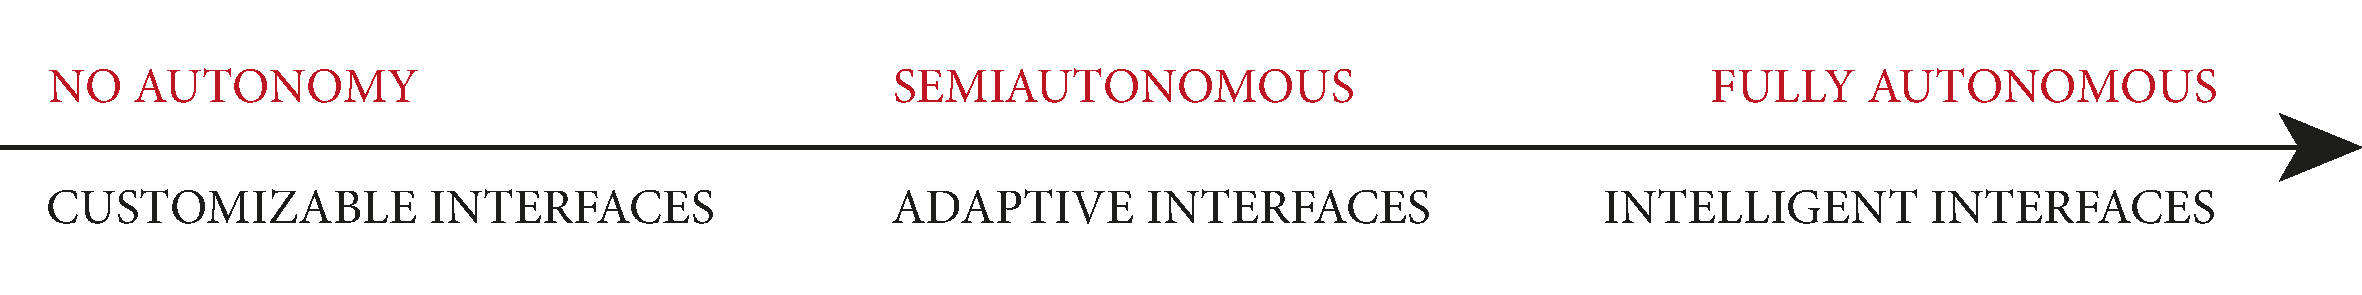
\includegraphics[width=\textwidth]{../graphics/autonomy.pdf}
  \caption[Levels of Interface Autonomy]{
    Levels of Interface Autonomy:
    Interfaces range from those only customizable by the user, 
    to intelligent systems takes the initiative on their own accord.
  }
  \label{fig:autonomy}
\end{figure}

Using AI to adapt an interface raises important questions with regard to usability, privacy and usefulness.
These questions are rooted in the autonomy expressed by each interface.
An autonomous interface is one that takes initiatives on its own, regardless of whether the user has asked for it \cite[p2]{Lieberman}. 
Naturally, any application that automatically personalizes its content will be autonomous to some degree.

Adaptive interfaces can be classified into increasing order of autonomy (see Figure \ref{fig:autonomy}). 
At the order of least autonomous systems, we have \emph{customizable interfaces}. 
These are interfaces that the user may customize themselves, but that do not take the initiative or change anything without explicit user action. 
For example, an interface might have a settings panel where users can change the order of items in a menu.
At the next level of autonomy, we have \emph{adaptive interfaces} that suggest to the user possible changes or actions that might be beneficial. For example, an email application could suggest which folder an email should be moved to.
At the most autonomous level, \emph{intelligent interfaces} implicitly and automatically customize the interface or content based on passive observation of the user. 
This could for instance entail automatic filing of emails based on content classification and data mining of previous user actions with similar messages.

An application that personalizes content automatically will fall somewhere in the two last categories and present either an adaptive or intelligent interface, 
depending on the extent and transparency of its autonomy.
We are only interested in fully atonomous, intelligent interfaces.
We wish to create a system that implicitly, and without any effort from each user,
can adapt the content of an application based on previous behaviour
Examples of implicit user modeling include \cite{Qiu2006}, \cite{Shen2005} and \cite{Carmel2009}.


\subsection{Aspects of Recommender Systems}

Formally, a recommender system can be seen as a quintuple, 
$\mathrm{RS} = (I, U, R, F, M)$,
where $I$ is the set of items (e.g. products, articles or movies) and 
$U$ is the set of users.
$R$ is the set of known ratings or utility, for example explicit preferences given by users for certain items, or connections in a social graph.
We have explicit ratings whenever the user provides their own ratings (e.g. product purchases),
and implicit ratings when the system infers ratings from behaviour (e.g. query log mining).
$F$ is a framework for representing the items, users and ratings, for example a graph or matrix. 
$M$ is the actual user modeling algorithm used to infer unknown ratings 
for predicting a user's preference for an unrated item. This is where AI comes in.

In \citet[p2]{Adomavicius2005}, $M$ is seen as a utility (the rating, in AI terms) estimation function
$p: U \times I \rightarrow S$. Here, $p$ (for prediction) is a function that maps the set
of users and items into a fully ordered set of items $S$, ranked by their
utility to each user. In other words, $S$ is the completely specified version of $R$,
where each user has either an explicit, implicit or predicted preference for each item in $I$.
To predict the best unrated item for each user, we simply find the item with the highest expected utility:

\begin{eqsp}
  \forall u \in U,\text{ } i'_u = \arg\max_{i \in I} p(u,i)
\end{eqsp}
%
The utility function $p$ depends on the modeling method being used, the active user and the item in question. 
The \emph{reason} for using a recommender system is that the utility (each $r$) is not defined for the entire $U \times I$ space, 
i.e. the system does not explicitly know the utility of each item for each user. 
The point of a recommender system is then to extrapolate $R$ to cover the entire user-item space. 
In other words, to be able to rank items according to user preferences, 
the system must be able to predict each user's reaction to items they have not yet explicitly or implicitly rated themselves. 

Another popular way of describing and implementing an RS is using a simple matrix.
This is what we shall use in this paper. 
In this matrix, one dimension represents users and the other represents items.
Each populated cell corresponds to an known rating. 
This matrix then becomes the framework $F$ in our RS quintuple:

\begin{eqsp}
 R_{u,i} =
 \begin{pmatrix}
  r_{1,1} & r_{1,2} & \cdots & r_{1,i} \\
  r_{2,1} & r_{2,2} & \cdots & r_{2,i} \\
  \vdots  & \vdots  & \ddots & \vdots  \\
  r_{u,1} & r_{u,2} & \cdots & r_{u,i}
 \end{pmatrix}
\end{eqsp}
%
Critically, these matrices are usually extremely sparse (most of the cells are empty). 
While there may be a large number of users and items, each individual user
only rates or connects to a few number of items.
This is true for any scenario where users rate items, access items in search results,
or connect to each other in a social network. 
For example, in the seminal Netflix Challenge movie recommender dataset, almost 99\% of the potential
user/item pairs have no rating \cite[p1]{Bell2007d}. In other words, 
this recommender system had to be able to produce results from a matrix where only 1\% of the cells have meaningful values.

This is the defining characteristic of many recommender systems: 
their ability to extract meaningful patterns from sparse data, 
through dimensionality reduction, neighborhood estimation and many other methods, as we shall soon see.
Naturally, much research looks at ways to best tackle this sparsity
(e.g. \cite{Pitsilis2009}, \citet[p3]{Claypool1999}, \citet[p19]{Ziegler2005}).

Recommender systems face many challenges other than this sparsity problem.
A directly related problem is the need for large datasets. Since the data is often sparse,
the systems will most often perform well if used on large numbers of items and users.
As in many machine learning methods, concept drift \cite[p1]{Widmer1996}, where the characteristics of a user or item
changes over time, is also always present.

The performance of RSs is often closely tied to their computational complexity
(as mentioned in \citet[p6]{Adomavicius2005}). 
Real world usage of the most precise methods is often hindered by the computational power
needed to actually put them into production.

Finally, the scale of the data in question should be a concern. If the ratings are ordinal data (e.g. 1-5)
input directly by users, the RS should take into account the domain specific meaning of these intervals.
For example, in a system for rating movies, the jump between ratings 4-5 might not have the same significance as
the jump from 2-3. However, this is a fact seldom mentioned in the literature. Most RSs 
employ metrics that assume a normal distribution, and even the common
evaluation techniques such as RMSE or MAE treat ordinal data as a continous scale.
We will get back to this in Chapter \ref{chap:discussion}. 
% http://technocalifornia.blogspot.com/2011/04/recommender-systems-were-doing-it-all.html


\subsection{Predicting Ratings}

The crucial part of any RS is how it predicts unknown ratings.
Because of this, each method is best categorized based on dimensions of its predictive capabilities (see Table \ref{table:taxonomy}).
We use a taxonomy where these dimensions are: 
available \emph{data}, 
prediction \emph{method}, 
model \emph{granularity}, 
knowledge \emph{temporality} and 
knowledge gathering \emph{agents}.

\begin{table}[b]
  \begin{tabular*}{\textwidth}{ p{3cm} l @{\extracolsep{\fill}} }
    \toprule
    \emph{Variable} & \emph{Possible values} \\
    \midrule
    Data & Content-based | Collaborative | Hybrid\\
    Method & Heuristic | Model-based\\
    Granularity & Canonical | Typical | Individual\\
    Temporality & Short-term | Long-term\\
    Agents & Implicit | Explicit\\
    \bottomrule
  \end{tabular*}
  \caption[Recommender Systems Taxonomy]{A taxonomy of recommender systems. From \cite{Bjorkoy2010d}.}
  \label{table:taxonomy}
\end{table}

The \emph{data} variable represents what data an RS uses to perform predictions. 
Content-based methods use only items, intra-item relations, and 
an individual user's past history as predictive of future actions \cite[p1]{Pazzani2007}.
By only considering the individual user in adapting an application, highly personal models can be created. 
However, such methods often require a lot of interaction before reliable models can be created \cite[p4]{Adomavicius2005}.
The problem of having to do complex inference from little data, as is often is in content-based predictions, i
similar to the \emph{sparsity problem}, is often called the \emph{cold start} or \emph{new user} problem. 
This is closely related to the common AI problem of \emph{overfitting} data, 
where the algorithms creates models that match the training data, 
but not the actual underlying relationships. 
As with the sparsity problem, a lot of research looks at ways to overcome sparse data, i.e. achieving "warmer" cold start
(e.g. \cite{Said2009}). 
When using content-based predictions, the utility function $p(u,i)$ of user $u$ and item $i$ is extrapolated from $p(u,i_x)$, 
where $i_x$ is an item similar to $i$ and $p(u,i_x)$ is known \cite[p2]{Adomavicius2005}.

Collaborative or social recommendations build predictive models for users based on the actions of similar users 
\citep{Schafer2007}.
The observation is that similar users should have similar usage and action patterns. 
By using data from more than one user, expansive models may be built. 
These methods are especially useful when considering new users of a service. 
A central problem with collaborative methods is that the resulting model is not as individually tailored as one created through content-based prediction. 
Collaborative models must be careful not to represent the \emph{average} user, but a single individual.
When using a collaborative method, 
the utility $p(u,i)$ of item $i$ for user $u$ is extrapolated from $p(u_x,i)$ where $u_x$ is a user similar to $u$
\cite[p4]{Adomavicius2005}. 

Because of \emph{the new user problem} of content-based prediction and the \emph{average user problem} of collaborative prediction, 
many systems use a hybrid approach (as introduced by \cite{Burke2007}).
By combining content-based and collaborative methods, 
systems that properly handle predictions for new users and avoid too much generalization in the models can be achieved. 

The \emph{method} variable, is another way to classify recommenders. Orthogonal to what data the method uses, this variable
concerns \emph{how} the data is used to produce recommendations.
First we have the \emph{model-based} approach, where the recommender system builds predictive models based on the known data. 
Unseen items can then be fed into this model to compute its estimated utility score
\cite[p5]{Adomavicius2005}. 
For example, creating a Bayesian networks from past interaction is a model-based approach.
The other category is the \emph{heuristic} or \emph{memory-based} approach \cite[p5]{Adomavicius2005}. 
These methods use the raw data of items, users and ratings to directly estimate unknown utility values. 
For example, recommending items similar to the ones already rated by computing the cosine similarity of their feature vectors is a heuristic approach.

The \emph{granularity} variable tells whether this approach creates models for the canonical user, stereotypical users or individual users. 
For example, \cite{Rich1979} presented one of the first user modeling systems based on stereotypes, 
used to predict which books in a library each user would most enjoy.
Here, a dialogue between the system and the user was performed to place the user into a set of sterotypes. 
Each stereotype has a set of \emph{facets} which is then used to match books and users.
This created user models of \emph{typical} granularity, as opposed to common \emph{individual} approaches.

\emph{Temporality} refers to how volatile the gathered knowledge will be.
While most RSs produce long term, relatively stable knowledge based on lasting user preference and taste, 
some systems use fluctuating parameters such as the time of day, exact location and the current context to produce recommendations.
For example, \cite{Horvitz} used clues from a user's calendar, camera and other sensors to determine the attentional state
of the user before delivering personalized and contextual notifications.

The \emph{agents} variable signifies whether the knowledge gathering and presentation is implicit and opaque, 
or explicit and requires dedicated user interaction. Explicit feedback through ratings is 
common in movie, product or music rating services (e.g. \cite{Bell2007, Basu1998, Hotho}). However, for other services such as personalized search,
implicit mining of query logs and user interaction is often used to build user models (e.g. \cite{Shen2005, Agichtein2006, Speretta2000, Teevan2005})


\subsection{Examples of Recommender Systems}
\label{subsec:recommender:examples}

As our solution will combine different recommender systems, we need a short introduction to some of the approaches we will use.
Let us take a closer look at (1) \emph{baseline ratings}, (2) \emph{neighborhood estimation}, (3) \emph{dimensionality reduction}, 
and (4) \emph{network traversal}. This is by no means an exhaustive list, but rather
a quick rundown of common approaches in recommender systems, that we will use in the Chapter \ref{chap:methods}.
See \cite{Adomavicius2005}, \cite{Pazzani2007}, \cite{Schafer2007} or \cite{Bjorkoy2010d} for a more comprehensive exploration of different types of recommenders.
\cite{Segaran2007} gives a good introduction to how RSs are used in practice.

(1) \emph{Baseline ratings} are the simplest family of recommender systems, based on rating averages.
The data is content-based, and used to compute heuristic predictions.
While simple in nature, they are often helpful as starting points for more complex systems, or as 
benchmarks for exploring new approaches. \cite[p2]{Koren2008} computes the baselines for items and users, and
use more involved methods to move this starting point in some direction. 
The baseline for a user/item pair is given by

\begin{eqsp}
  b_{ui} = \mu + b_u + b_i
\end{eqsp}
%
where $\mu$ is the average rating across all items and users, 
$b_u$ is the user baseline and 
$b_i$ is the item baseline.
The user and item baselines correspond to how the user's and item's ratings deviate from the norm.
This makes sense as some items may be consistently rated higher than the average, some users may be 
highly critical in their assesments, and so on. \citeauthor{Koren2008} computes these baselines by solving the
least squares problem

\begin{eqsp}
  \min_{b*} = \sum_{(u,i) \in R} (r_{ui} - \mu - b_u - b_i)^2 + \lambda ( \sum_{u} b_u^2 + \sum_{i} b_i^2 )
\end{eqsp}
%
which finds baselines that fit the given ratings while trying to reduce overfitting
by punishing greater values, as weighted by the $\lambda$ parameter. 
By using baselines instead of simple averages, more complex predictors gain a better starting point,
or in other words, a better average rating.

Another approach based on simple averages is the  \emph{Slope One} family of recommender algorithms. 
As introduced by \cite{Lemire2005}, these algorithms predict unknown ratings based on the average difference in ratings between two items. 
For example, if item $i$ is on average rated $\delta$ points above item $j$, and the user $u$ has rated item $j$,
that is, we know $r_{uj}$, the predicted rating of $i$ is simply $r_{uj} + \delta$, for all ratings that match this pattern.
In other words,

\begin{eqsp}
  \hat{r}_{ui} = \frac{\sum_{j \in K_u} \mathrm{ratings}(j) \times (r_{uj} + \mathrm{diff}(i,j))}{\sum_{j \in K_u} \mathrm{ratings}(j) },
\end{eqsp}
%
where $\hat{r}_{ui}$ is the estimated rating, $K_u$ is the items rated by user $u$, $\mathrm{ratings}(i)$ is the number of ratings for item $i$,
and $\mathrm{diff}(i,j)$ is the average difference in ratings for items $i$ and $j$.
While simplistic, Slope One is computationally effective and produces results comparable to more complex methods \cite[p5]{Lemire2005}.

(2) \emph{Neighborhood estimation} is part of many recommendation systems. 
It is the core principle behind most collaborative filtering algorithms, that
estimate an unknown rating by averaging the ratings of similar items or users, weighted by their similarity.
These approaches often work in two steps: First, a neighborhood if similar elements is computed.
Second, the similarities and connections within this neighborhood is used to produce a prediction.

The principal method for computing user similarity is the \emph{pearson correlation coefficient} (PCC)
\cite[p11]{Segaran2007}.
While simple, the PCC compares favorably to more complex approaches, and is often used as a benchmark 
for testing new ideas (e.g. in \citet{Lemire2005, Ujjin, Konstas}).

The PCC is a statistical measure of the correlation between two variables. In our domain, the variables
are two users, and their measurements are the ratings of co-rated items. 
The coefficient produces a value in the range $[-1,1]$ where $1$ signifies perfect correlation (equal ratings),
$0$ for no correlation and $-1$ for a negative correlation.
The negative correlation can for example signify two users that have diametrically opposing tastes in movies.
We compute PCC by dividing the covariances of the user ratings with their standard deviations:

\begin{eqsp}
  \mathrm{pcc}(u,v) = \frac{cov(R_u, R_v)}{\sigma_{R_u} \sigma_{R_v}}.
\end{eqsp}
%
When expanding the terms for covariance and standard deviations, 
and using a limited neighborhood size $n$, we get

\begin{eqsp}
  \mathrm{pcc}_{n}(u,v) = 
    \frac{
      \sum_{i \in K}^{n} (R_{ui} - \bar{R_u}) (R_{vi} - \bar{R_v}) }{ 
        \sqrt{ \sum_{i \in K}^{n} (R_{ui} - \bar{R_u})^2 } 
        \sqrt{ \sum_{i \in K}^{n} (R_{vi} - \bar{R_v})^2 }}.
\end{eqsp}
%
The limited neighborhood size becomes the statistical sampling size, and is a useful
way of placing an upper bound on the complexity of computing a neighborhood.
$n$ does not have to be a raondom sampling --- it can also be limited by the number of ratings 
the two compared users have in common, the number of ratings each user have, or something similar,
as denoted by $K$ in our the formula.

After a neighborhood is determined, it is time to predict our desired rating.
When using \emph{collaborative} recommenders, this means averaging the neighborhood ratings weighted by similarity \cite[p16]{Segaran2007}:

\begin{eqsp}
  \bar{r}_{ui} = \frac{ \sum_{v \in K(u,i)} \mathrm{sim}(u,v) \times R_{vi} }{ \sum_{v \in K(u,i)} \mathrm{sim}(u,v) },
\end{eqsp}
%
where $\mathrm{sim}(u,v)$ is the similarity between two users, $K(u,i)$ is the set of users in the neighborhood of $u$ that have rated item $i$.
This is possible the simplest way of computing a neighborhood-based prediction.
Most systems use more complex estimations. For instance, \cite{Koren2008} 
uses the baseline ratings discussed above instead of plain user and item ratings, to
remove what they call global effects where some users are generous or strict in their 
explicit preferences, and some items are consistently rated differently than the average.

\emph{Content-based} recommenders based on neighborhoods work on similar principles.
The difference is that we compute similarities between items, not users. The simplest
approach is to find items highly rated by the current user, compute the neighborhood 
by finding items similar to these, and produce ratings by weighting the initial rating
with the similarity of the neighboring items.

The PCC is but one of many methods used to compute neighborhoods. 
Other simple measures include the \emph{euclidean distance} \cite[p10]{Segaran2007},
Spearman's or Kendall Tau rank correlation coefficients \cite[p30]{Herlocker2004} --- 
variations on the PCC.
Of course, user similarity does not have to rely on ratigs. 
If the system has access to detailed user profiles, these can be used
to estimate the similarity of users.
Similarity metrics from information retrieval,
such as \emph{cosine correlation} from the \emph{vector space model} (VSM) are also popular,
used to compute item similarities (see section \ref{sec:search}).

\cite{Bell2007a} shows a more sophisticated neighborhood estimation which computes global interpolation weights,
that can be computed simultaneously for all neirest neighbors.
Combinations of metrics are also possible: 
\cite{Ujjin} first use a simple euclidean metric to gather a larger neighborhood, which is then refined
by a \emph{genetic algorithm}.
Another way of computing neighborhoods is by reducing the dimensions of the ratings matrix,
as we will now describe.


(3) \emph{Dimensionaliy reduction} is an oft-used technique when creating recommender systems.
The ratings matrix is factored into a set of lower dimension matrixes, that can be used to approximate the original matrix.
Since this has the added effect of trying to approximate unknown cells, the lower dimension matrices
can be used to predict unknown ratings (a type of least squares data fitting).

\emph{Singular Value Decomposition} (SVD) is a common method for such matrix factorization (e.g. \citet[p5]{Billsus}, \citet{Sun2005}, \citet{Bell2007}).  
This is the same underlying technique used by \emph{latent semantic indexing} (LSI) in information retrieval \cite[p44]{Baeza-Yates1999}.
Formally, SVD is the factorization $M = U \Sigma V^{T}$. 
$M$ is an $m \times n$ matrix, in our case the ratings matrix, with $m$ users and $n$ items. 
$U$ is an $m \times m$ factor (sometimes called the "hanger"), $V^{T}$ (the transpose of $V$) is an $n \times n$ factor (the "stretcher").
$\Sigma$ is a $m \times n$ diagonal matrix (the "aligner"). 
$\Sigma$ is a diagonal matrix, made up of what is called the \emph{singular values} of the original matrix.

The dimensionalty reduction can be performed by truncating the factor matrices each to a number of rows or columns, 
where the number is a paramenter depending on the current domain and data, called the $rank$ ($r$).
The truncated matrix is $M_r = U_r \Sigma_r V_r^{*}$, where $U_r$ are the first $r$ columns of $U$,
$V_r^{T}$ are the first $r$ rows of $V^{T}$ and $\Sigma_r$ is the top-left $r \times r$ sub-matrix of $\Sigma$.
There are many more complex ways of compressing the matrix than pure truncation, but this is the most 
common way of reducing the factors.
By truncating the factors, 
we in essence create a higher-level approximation of the original matrix that can identify latent features in the data.
With the factors reduced to $r$ dimensions, the result looks like this:

\begin{eqsp}
  \begin{bmatrix}
    { } & { } & { }     & { } & { }\\
    { } & { } & { }     & { } & { }\\
    { } & { } & R_{m,n} & { } & { }\\
    { } & { } & { }     & { } & { }\\
    { } & { } & { }     & { } & { }
  \end{bmatrix} 
  \quad 
  \Rightarrow
  \quad
  \begin{bmatrix}
    { }\\
    { }\\
    U_{m,r}\\
    { }\\
    { }
  \end{bmatrix}
  %\quad
  \begin{bmatrix}
    \Sigma_{r,r}
  \end{bmatrix}
  %\quad
  \begin{bmatrix}
    { } & { } & V_{r,n}^{*} & { } & { }\\
  \end{bmatrix} 
\end{eqsp}
%
Two important transformations happen in this dimensionality reduction. 
First, ratings that do not contribute to any greater pattern are removed as "noise".
Second, ratings that in some way correlate to each other are enhanced, giving more weight to the actual predictive parts of the data.
This means that the reduced factors can for instance identify features that correspond to correlations between items or users.
These features are comparable to the mapping of terms to concepts in LSI.

\begin{figure}[t]
  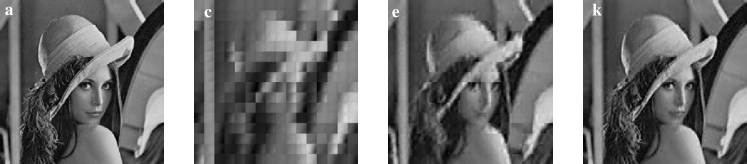
\includegraphics[width=\textwidth]{../graphics/compression}
  \caption[SVD Image Compression]{
    SVD Image Compression:
    A variation of using SVD to compress an image, from \cite{Ranade2007}.
    The original image is on the left, and successive images use an increasing number of factors (2, 8 and 30) when performing compression.
    Figure adapted from \citet[p4]{Ranade2007}.
  }
  \label{fig:svd-image}
\end{figure}

Because SVD can find the most descriptive parts of a matrix, this technique is often used for image compression.
The image we wish to compress is treated as an $N \times M$ matrix, which is run through an SVD factorization.
The factors are truncated, and the result expanded to a matrix that is much simpler to represent
than our original image matrix. As seen in Figure \ref{fig:svd-image}, how close the compressed image resembles the original image
depends on the chosen $rank$, i.e. how many rows and columns we keep during truncation.
A higher rank means less dimensionality rediction and less compression of the image.

In recommender systems, SVD is used to compress the ratings space into what is sometimes called a \emph{taste space},
where users are mapped to higher-level "taste" categories
(e.g. \citet[p5]{Ahn2004}, \citet[p4]{Brand2003} or \citet[p2]{Liu2006}).
In a taste space,
the collections of individual ratings are reduced to groups of users, items and combinations that have patterns in common.
This reduction makes it easy to find similar users that share some global characteristic.
We can of course also find similarities between items, clusters of items and user and so on, all based on latent "categories"
discovered by the automatic identification of patterns in the data.
SVD is then an ingenious way of dealing with the commonly sparse ratings data, by identifying latent correlations and patterns in the data,
which is exactly what we need to predict unknown ratings or connections.

(4) \emph{Network traversal} refers to estimating predictions by traversing a graph of users and items to provide recommendations.
The connections between nodes can be any type of relation that makes sense to the RS. Examples include linking item and user nodes
based on purchases or explicit ratings, linking user nodes from asymetrical (directed edges) symetrical (undirected edges) relations,
or linking items based on some similarity metric.
Recommender systems can use common graph-traversal algorithms to infer unknown connections in this graph.

\cite{Huang2002} used network traversal to create a simple system for recommending books to customers.
Here, edges between items and users correspond to ratings, and edges connecting nodes of the same type
are created by connecting elements that have similarity above a certain threshold. Predictions are generated
by traversing the graph a preset number of steps starting at the current user, and multiplying the weights
of paths leading to the target item (see Figure \ref{fig:book-graphs}).

\begin{figure}[t]
  \centering
  \subfloat[]{\label{fig:graph-layers}
    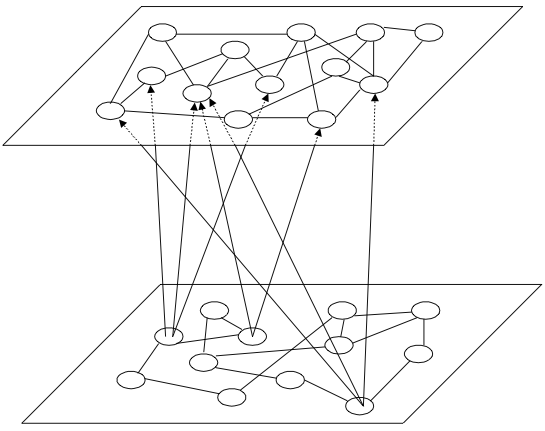
\includegraphics[width=0.5\textwidth]{../graphics/graph-layers}}                
  \subfloat[]{\label{fig:graph-layers-detail}
    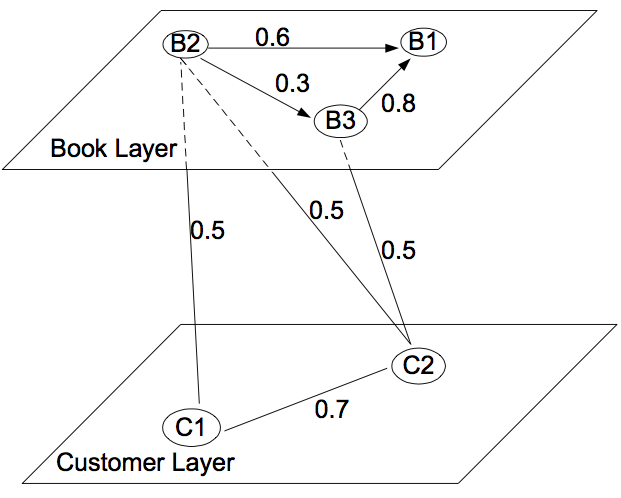
\includegraphics[width=0.5\textwidth]{../graphics/graph-layers-detail}}
  \caption[Network Traversal]{Network Traversal: (a) A graph with two kinds of nodes,
    e.g. items and users. (b) A graph with books and customers, where recommendations
    can be made by traversing the weighted connections. Connections between nodes of the same type
    represent similarity, while connections between books and customers represent purchases.
    Figures from \cite{Huang2002}.}
  \label{fig:book-graphs}
\end{figure}
%
The complexity of recommender systems based on networks are only limited by the kinds of relations we can produce.
For example, recommending other users in social networks can easily utilize friend or friend-of-a-friend relations
to find others the current user might be interested in connecting to. Indeed, any relevant similarity metric can be used to
connect nodes of the same type, or nodes of different types.

One variation comes from \cite{Walter2008}, who create a network of \emph{transitive trust} to produce recommendations. Here,
the neighborhood of users is determined by traversing through users connected by a level of trust. 
The trust can for example be a function of how many agreeable results the connection to a user has produced.
In other words, users trust each others recommendations based on previous experience.

\cite{Konstas} takes yet another approach that measures the similarity between two nodes through their \emph{random walks with restarts} (RWR) technique.
Starting from a node $x$, the RWR algorithm randomly follows a link to a neighboring node. 
In every step, there is a probability $\alpha$ that the algorithm will restart its random walk from the same node, $x$. 
A user-specific column vector $\mathbf{p}^{(t)}$ stores the long term probability rates of each node, 
where $\mathbf{p}^{(t)}_i$ represents the probability that the random walk at step $t$ is at node $i$. 
$\mathbf{S}$ is the column-normalized adjacency-matrix of the graph, i.e. the transition probability table. 
$\mathbf{q}$ is a column vector of zeroes with a value of $1$ at the starting node (that is, $\mathbf{q}_i$ is $1$ when the RWR algorithm starts at node $x$). 
The stationary probabilities of each node, signifying their long term visiting rate, is then given by 

\begin{eqsp}
  \mathbf{p}^{(t+1)} = (1 - \alpha)\mathbf{S}\mathbf{p}^{(t)} + {\alpha}\mathbf{q}
\end{eqsp}
%
when it is run to convergence (within a small delta). Then, the \emph{relatedness} of nodes $x$ and $y$ is given by $\mathbf{p}_y$ where $p$ is the user model for the user represented by node $x$.
\citeauthor{Konstas} found that this approach outperformed the PCC, as long as the social networks were an explicit part of the system in question.
In other words, the connections between users had to be one actively created by the users to be of such quality and precision that
accurate predictions could be made.

After this whirlwind tour of recommender systems, it is time to look at some closely related topics:
information retrieval and personalized search. This will form the basis for the case study
performed in the next chapter.


\section{Personalized Search}
\label{sec:search}

Personalized search means adapting the results of a search engine to each individual user.
As we shall see, this field has a lot in common with user modeling and recommender system.
In both situations, we wish to predict how relevant an item will be to each user.
Before delving into the techniques of personalizing search results, we present 
the basics of \emph{information retrieval} (IR).

\subsection{Information Retrieval}
\label{sec:ir}

\citet[p1]{Manning2008} define IR as "finding material (usually documents) of
an unstructured nature (usually text) that satisfies an information need
from within large collections (usually stored on computers)".

How does this relate to recommender systems? There is an important distinction:
The purpose of \emph{recommending} is twofold: (1) show the user items
similar to another item, and (2) allow discovery of relevant items the user did not know exist.
The purpose of \emph{search} is a bit different: allow the user to find the location of
information he or she knows (or hopes) exists.
In other words, the defining separator is often the knowledge of existence.
However, as we shall see in this chapter, the two fields employ a lot of the same
methods and terminology. In the next chapter, we will show how these can work together.

\citet[p23]{Baeza-Yates1999} presents a formal definition of an IR system:

\begin{eqsp}
  \mathrm{IR} = (Documents, Queries, Framework, ranking(q_i, d_i)).
\end{eqsp}
%
As evident by the scope of IR literature, these elements can be just about anything
that has to do with retrieving information. However, in what is often called
\emph{classic IR}, the documents contain free text with little to no describing structure,
and the queries are short user-initiated descriptions of an \emph{information need} \citep[p19]{Baeza-Yates1999}. 
Among other domains, this model describes web search engines, where the documents are web pages and
queries are short sentences or a few keywords input by users.

The \emph{Framework} in our quadruple refers to how documents are stored and retrieved.
Basic approaches to IR split each document into a set of terms (e.g. words),
and create an inverted index \cite[p22]{Manning2008} that lists each document that each term appears in.
There are numerous extensions to this framework, including: 

\begin{itemize*}
  \item Positional information for phrase search \cite[p39]{Manning2008}
  \item Stop word removal (removing the most common terms) \cite[p27]{Manning2008}
  \item Stemming (reducing words to their root forms) \cite[p32]{Manning2008}
  \item Lemmatization (contextual inflection removal) \cite[p32]{Manning2008}
  \item Query reformulation \citep[p117]{Baeza-Yates1999}
\end{itemize*}

All these techniques help improve (among other things)
the \emph{recall} and \emph{precision} of the retrieval engine. 
Recall, precision and relevance are well defined masures for evaluating the quality of a search engine \cite[p5]{Manning2008}:

\begin{itemize*}
  \item A document is \emph{relevant} if it satisfies the user's information need.
  \item \emph{Recall} is the fraction of relevant documents retrieved by the system.
  \item \emph{Precision} if the fraction of retrieved documents that are relevant.
\end{itemize*}

There are many more measures, but recall and precision succintly define what a search engine must to
to be successfull: retrieve many relevant documents and few irrelevant documents.
Failing this test is to neglect the main purpose of an IR:
preventing information overload by allowing people efficient access 
to relevant parts of an otherwise overwhelming information repository.

To us, however, the most interesting part of any IR system is the \emph{ranking function}.
This function maps queries to documents by a scalar score, signifying how well a match
each document is to a query. The relation to recommender systems should be self-evident,
and indeed, IR systems use many of the same metrics to measure query/document similarity.

A common framework for storing and ranking documents is the previously mentioned vector space model (VSM).
This model stores documents as term vectors. Each term represents a dimension, and documents are
vectors in this term-space. When performing a query, the query terms are also represented as a vector
in the same space. By computing the cosine similarity between the query and each document,
we get a good estimate of how well a document matches a query \citep[p29]{Baeza-Yates1999}.

The next question is what to store at each (document, term) coordinate in the vector space
(called the document-term weights).
Storing simple 1 or 0 values representing whether or not terms are present gives a model 
where a document's relevance is proportional to how 
many of the query terms it includes. However, this is not very precise. 
For example, by this definition, a document containing every conceivable query term
would be the most relevant to any query.
A better idea is to use something like the TF-IDF weighting scheme \citep[p29]{Baeza-Yates1999}:

\begin{eqsp}
  w_{t,d} = tf_{t,d} \times idf_{t}
          = \frac{ \mathrm{freq}(t,d) }{ \sum_{k \in d} \mathrm{freq}(k,d) } \times 
            \log \frac{N}{n_{t}}.
\end{eqsp}
%
The final weight is computed by multiplying the term frequency score (TF) $tf_{t,d}$ with the 
inverse document frequency (IDF) $idf_{t}$. TF evaluates how well the term describes the document contents,
while IDF punish terms that appear in many documents. 
$freq_{t,d}$ gives the frequency of a term in a document. $N$ is the total number of documents,
and $n_{t}$ the number of documents in which $t$ appears. The effect of the IDF factor is dampened by taking its
log-value. Together, TF and IDF ranks documents higher by words that discriminate well within the document corpus,
and ignores words that appear in so many documents that they have little to no predictive capacity.

While simple, TF-IDF has proven itself resilient when compared to more complex methods,
and many more complex methods have been built on its foundations (e.g. BM25, one of the most successfull
probabilistic weighting algorithms \citep{Robertson2010}).

There are as many IR models as there are domains that need search,
and even the basic vector space model can be constructed in a myriad of ways. There is also the simpler 
\emph{boolean search model}, where queries are based on boolean algebra. Probabilistic models
frame the similarity question as the probability that the document is relevant. 
Latent Semantic Indexing (LSI), the application of SVD to IR by performing dimensionality reduction of the term-space
into concept-space is another approach.
See \cite{Manning2008}, \cite{Robertson2010} or \cite{Baeza-Yates1999} for a more comprehensive introduction to models in IR.

The important take-away is that, while serving different use cases, RSs and IR systems 
employ much of the same technology with different input and expected output.


\subsection{Ranking Signals}
\label{subsec:signals}

Modern web search engines have long ago moved on from simple ranking metrics such as TF-IDF.
While similar traditional metrics may form the foundation of modern search engines, a lot more thought go into the final results.
Different types of rankings are combined to produce the final \emph{search engine results page} (SERP),
with each ranking function often being referred to as a \emph{signal}. Alternate names include
\emph{reranking} or \emph{rescoring} functions.

Google, the company behind the popular online search engine, writes: "Today we use more than 200 signals, including PageRank, 
to order websites, and we update these algorithms on a weekly basis. 
For example, we offer personalized search results based on your web history and 
location."\footnote{\url{google.com/corporate/tech.html} --- accessed 11/04/2011}
Bing, another popular search engine, uses the same terminology:
"We use over 1,000 different signals and features in our ranking 
algorithm."\footnote{\url{bing.com/community/site_blogs/b/search/archive/2011/02/01/thoughts-on-search-quality.aspx} --- accessed 11/04/2011}

Signals are often products of the document structure of the current domain.
\citet[p5]{Bender2005} points to the use of the proximity of query terms in matching documents.
Those where the terms appear close together are natural candidates for a higher ranking.
Other signals, still reliant on the documents themselves, are more domain oriented.
Another signal they point out is how words in a larger or bold font can be weighted 
higher than normally typset words.

Signals can also depend on the query. \citet[p145]{Manning2008} describes a system that takes
multi-word queries, breaks them up into different permutations and runs each new query against the same
document index and ranking function. Each query corresponds to its own ranked set of results,
which are sent to a \emph{rank aggregation function} which turns the accumulated ranking evidence
into one coherent result. We will have more to say on rank aggregation in Section \ref{sec:aggregate}.  

Signals can also be external to the collection or relational within the collection.
PageRank \cite[p4]{Bender2005} is perhaps the most known of the relational signals.
The algorithm forms a probability distribution over web pages, ranking their percieved
authority or importance according to a simple iterative estimation.
Each web site is given its rank based on how many pages that link to it.
For each page that provides links, the score it contributes to the linked-to page is 
its own page rank weighted inversely proportional to the number of outbound links the page has.
Another intuitive justification for a site's PageRank is the \emph{random surfer model} \cite[p4]{Bender2005}.
The probability that the random surfer visits a page is its PageRank. The "randomness" is introduced 
by a damping parameter $d$, which is the probability that a user will stop browsing and start at a new random page:

\begin{eqsp}
  \mathrm{PageRank}(x) = \frac{1 - d}{N} + d \sum_{y \in B_x} \frac{\mathrm{PageRank}(y)}{\mathrm{Links}(y)},
\end{eqsp}
%
where $B_x$ is the set of pages linking to page $x$, and $\mathrm{Links}(y)$ is the number of outbound links from page $y$.
The first term distributes an equal pagerank score to all pages that have no outbound links, as $N$ is the total number of pages.
This iterative algorithm is run until convergence inside a small delta.

Let us now finally take a look at one of the main uses of signals: \emph{personalized search}.


\subsection{Personalizing Search Results}

Search engines, especially online search engines, face a huge challenge. 
In addition to the wide range of websites, the ambiguity of language,
the restricted nature of queries, comes the wildly differing users.
Each user is unique. Even when considering one user, there might be many 
different use cases, for example when using the same search engine at work and at home.
Another identified problem is that users use search engines for navigation as well as pure search.
\citet{Teevan2007} found that as many as 40\% of all queries to the Yahoo! search engine were "re-finding queries",
i.e. attempts to find information the user had accessed before.

\emph{Personalized search} (PS) attempts to solve these problems by introducing individually catered search results. 
These techniques are based on user modeling (as introduced in Section \ref{sec:modeling}),
and attempts to build predictive models based on mined user preferences.
Commonly, this is done through query log analysis (e.g. \cite{Liu2002, Sugiyama2004, Shen2005, Speretta2000})
In other words, these are often model-based techniques with implicit knowledge gathering agents,
that create individual, long-term user models (see Section \ref{sec:recommender}).

There are two leading approaches to personalizing search results \cite[p2]{Noll2007}. 
The first method is query reformulation, where the actual user query is enhanced in some way, before traditional IR 
retrieves and ranks documents. The second method is results re-ranking, where the IR results are sorted
based on personalized metrics. This section describes the latter approach.

To demonstrate how these methods compare to traditional recommendation systems,
we will explore a few different approaches to personalized search: 
(1) \emph{personalized topic-sensitive PageRank},
(2) \emph{folksonomy-based personalization} and
(3) \emph{social network search ranking}.

(1) \citet{Haveliwala2003} introduced a topic-sensitive PageRank algorithm, that they found
to be "generate more accurate rankings than with a single, generic PageRank vector". 
In essence, they create topic-specific PageRank vectors for a number of pre-set topics,
creating many rankings per page, one for each topic.
This new PageRank is computed based on an existing set of websites that belong to each topic.
\citet{Qiu2006} achieved "significant improvements" to this approach by adding a personally adaptive layer
to the topic-sensitive PageRank algorithm, creating a \emph{personalized PageRank algoriithm}. 

In addition to the topic vector, \citeauthor{Qiu2006}
creates a topic-preference vector for each user. When the user has clicked on a few search results,
a learning algorithm kicks in and estimates approximately how likely the user is to be interested 
in each of the pre-set topics, creating the topic-preference vector $T$. When it is time to rank a 
page $p$ in response to the query $q$, they compute the personalized ranking:

\begin{eqsp}
  PersonalizedRanking(T,p,q) = \sum_{t=1}^{m} T(i) \cdot Pr(q|T(i)) \cdot TSPR_i(p)
\end{eqsp}
%
We will not deduce this equation here (see \citet[p5]{Qiu2006}), but let us explain it. 
$T$ is the user-specific topic preference vector.
$i$ is the index of a topic and $m$ the total number of topics.
$Pr(q|T(i))$ is the probability that the query belongs in topic i.
This can be as simple as the total number of times the query terms appear in websites under topic $i$.
$TSPR_i(p)$ is the topic-sensitive PageRank score for page $p$ in topic $i$. Basically, this is 
the normal PageRank vector computed within a pre-set topic $i$.

The construction of $T(i)$, i.e. the training phase of the algorithm, is performed by mining the query logs for each user.
By identifying how many sites the user has visited in each topic, computing $T$ can be done through linear regression or
by using a Maximum-likelihood estimator (basically, any method that can fit a curve).
\citet[p10]{Qiu2006} reports improvements of 25\% to 33\% over the Topic-sensitive PageRank approach, which 
\citet{Haveliwala2003} reports outperformed the original PageRank algorithm.

%Cube svd: \cite{Sun2005}

(2) Web applications often have more information about users and items (documents, sites or articles) 
than simple ratings. One of these extra resources are tags, simple keywords assigned from users to items. 
The collection of users, items, tags and user-based assignment of tags to resources is called a \emph{folksonomy}.

\cite{Hotho} defines a folksonomy as a tuple $F = (U,T,R,Y,\prec)$. 
Here, $U$, $T$ and $R$ are finite sets of users, tags and resources (items), respectively. 
$Y$ is a ternary relation between users, tags and resources, called tag assignments. 
$\prec$ is a user-specific tag hierarchy, applicable if the tags are organized as super- and sub-tags. 
The \emph{personomy} $P_u$ is a user-specific part of $F$, 
i.e. the tags, items and assignments related to one user $u$. 
In our terms, this personomy would be the user model. 
\citeauthor{Hotho} use folksonomies to do information retrieval based on their 
\emph{FolkRank} search algorithm, a derivative of PageRank. 

\cite{Bao2007} shows how folksonomies can be used to personalize search.
They first create a topic-space, where every user and document are represented.
Each tag in the system is a dimension in this topic-space, or tag-space.
Whenever a new query is issued, two things happen: First, a regular IR method
computed a standard, non-personalized ranking of documents.
Second, a personalized ranking list is computed by performing a simple
vector-space model matching in the topic-space, for example by using
cosine similarity (as previously explained). The personalized list
is then unrelated to the actual query, and is simply a ranking of the
most relevant pages to the current user.

The two ranks are aggregated by a simple consensus-metric, the
\emph{weighted borda-fuse} (WBS) aggregator \cite[p3]{Xu2008}, 
which is nothing more than a weighted combination of the rankings:

\begin{eqsp}
  \mathrm{rank}(u,q,p) = \alpha \cdot \mathrm{rank}_{IR}(q,p) 
                 + (1-\alpha) \cdot \mathrm{rank}_{personal}(u,p)
\end{eqsp}
%
\citeauthor{Xu2008} tried many combinations of weights,
topic selection and datasets, with the general conclusion
that folksonomy-based personalized search has great potential.
If nothing else, this example shows how easily tags can be integrated
to provide an individual searching experience.

(3) \cite{Carmel2009} developed a personalized search algorithm based on a user's \emph{social network}.
By re-ranking documents according to their relation to with individuals in the current user's social network,
they arrived at a document ranking that "significantly outperformed" non-personalized social search \cite[p1]{Carmel2009}.
Note, however the qualifier "social search" --- their project searches through social data within an enterprise, 
naturally conducive to algorithmic alterations based on social concepts. However, as social data is data just as well,
seeing how a personalized approach improves standard IR in this domain, is helpful.

Their approach: First, documents are retrieved by a standard IR method. Second, the user's socially connected peers
are also retrieved. Third, the initial ranked list of documents is re-ranked based on how strongly they are connected 
to the user's peers, and how strongly those peers are connected to the user. The user-user similarity is
computed based on a few signals \cite[p2]{Carmel2009}, e.g. co-authoring of documents, the use of similar tags
(see (2)) or commenting on the same content. 
The user model also includes a list of terms the current user has employed in a social context (profile, tags, et cetera).
This is all done to infer implicit similarity based on social connections.

The algorithm is quite powerful, and combines three types of rankings: 
The initial IR score, the social connection score, and a term score, where the terms are tags and keywords used by a user.
The user model is $U(u) = (N(u), T(u))$, 
where $N(u)$ are the social connections of $u$ and $T(u)$ the user's profile terms.
First, the score based on connections and terms is computed, weighted by $\beta$ which determines the weighting of both approaches:

\begin{eqsp}
  S_P(q,d|U(u)) = \beta \sum_{v \in N(u)} w(u,v) \cdot w(v,d) + (1-\beta) \sum_{t \in T(u)} w(u,t) \cdot w(t,d)
\end{eqsp}
%
Finally, the results are combined with the ranking returned by the IR method ($R_{IR}$). 
A parameter $\alpha$ is used to control how much each method is weighted:

\begin{eqsp}
  S(q,d|P(u)) = \alpha \cdot R_{IR}(q,d) + (1-\alpha) \cdot S_P(q,d|U(u)) 
\end{eqsp}
%
This approach, while simple, shows how social relations and social annotations can easily be used to personalize a search experience.
However, \citet[p10]{Carmel2009} notes that the high quality data in their enterprise setting were important
to achieve the improved results. 





\section{Aggregate Modeling}

\begin{eqnarray}
  \mathrm{AM} = (Items, Users, Framework, Methods, Aggregation)
\end{eqnarray}




Use cases (netflix, ...)

For personalized search (speculation)

Hypotheses

Explain next chapter



 
\hr

This chapter has introduced the basic theory we will need to develop our take on user modeling.
The next chapter will build this model,
While Chapter \ref{chap:results} presents our evaluation experiments.


